\documentclass[tikz,border=5mm]{standalone}
\begin{document}
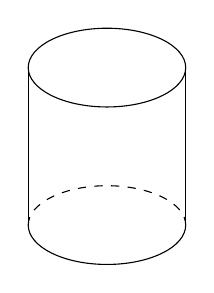
\begin{tikzpicture}
    % 绘制圆柱体
    \draw [dashed] (1,0) arc (0:180:1cm and 0.5cm);
    \draw (-1,0) arc (180:360:1cm and 0.5cm);
    \draw (1,2) arc (0:360:1cm and 0.5cm);
    \draw (-1,0) -- (-1,2);
    \draw (1,0) -- (1,2);
    
%    % 填充圆柱体
%    \filldraw[fill=gray!20!white, draw=gray] (0,0) circle (1cm);
%    \filldraw[fill=gray!20!white, draw=gray] (0,2) circle (1cm);
%    \filldraw[fill=gray!20!white, draw=gray] (-1,0) -- (-1,2) -- (1,2) -- (1,0) -- cycle;
\end{tikzpicture}
\end{document}